\documentclass[english, openany]{iamthesis}
% changle "slovak" to "english" for english version of the thesis

%----------------------------------------------------------------%
% THESIS DATA

% thesis level {bc | ing | min | dis}
\def\thesislevel{bc}

% student name with title e.g. Ing. Martin Klaučo
\def\thesisauthor{Ivana Dukayová} 

% year of submmiting to AIS
\def\thesisyear{2024}

% registration number generated by AIS e.g. 19990-50920
\def\thesisnumber{184466-115979} 

% thesis type: BACHELOR|MASTER|DISSERTATION or in slovak 
% BAKALÁRSKA|DIPLOMOVÁ|DIZERTAČNÁ
\def\thesistype{BACHELOR}

% thesis title
\def\thesistitle{Touchless Drone Navigation via Hand Gestures}

% thesis supervisor including degrees e.g. Ing. Martin Klaučo, PhD.
\def\thesissupervisor{doc. Ing. MSc. Martin Klaučo, PhD.}

% study field (translate to english if neccesarry) e.g. "Riadenie Procesov" or
% "Process Control"
\def\thesisprogram{Process Control}

% Institute (translate to english if neccesary)
% e.g., "Institute of Information Engineering, Automation, and Mathematics"
\def\thesisinst{ Department of Information Engineering and Process Control}

% Title of the Acknowledgment
% For slovak write: "Poďakovanie" for English write: "Acknowledgment"
\def\thesisack{Acknowledgment}


% End THESIS DATA
%----------------------------------------------------------------%

%----------------------------------------------------------------%
%   Titles and other stuff                                       %
%----------------------------------------------------------------%
\author{\thesisauthor}
\title{\thesistitle}
\date{\today}
%\usepackage{layouts}
%\usepackage{layout}
\usepackage{hyperref}
%\usepackage[margin=1cm]{geometry}
\usepackage{tikz,pgfplots,pgf}
\usetikzlibrary{arrows.meta} % <-- Make sure this line is here
\usepackage{tikz-qtree}
\usetikzlibrary{matrix,shapes,arrows,positioning}
%----------------------------------------------------------------%
%   Let the document begin                                       %
%----------------------------------------------------------------%
\begin{document}
\let\cleardoublepage\clearpage % Prevents adding blank pages before new chapters

% ---------------------------------------------------------------%
% The Frontmatter  !! Do NOT change the structure !!             % 
%----------------------------------------------------------------%

\coverpage

\frontmatter
\pagenumbering{roman}

% include assignment generated by AIS system
\includepdf[pages=-]{content/zadanie.pdf}
% use this command only if your assignment has more than 2 pages
% \includepdf[page=2]{content/assignment.pdf}


% do not remove following commands
% do not following commands
\chapter*{\thesisack}
\markboth{}{}
\addcontentsline{toc}{chapter}{\thesisack}
I am deeply grateful to Ing. Patrik Valabek for his insightful advice while we worked on this project, reminding me there is no turning back now. His guidance was crucial in dealing with these changes and helped me navigate the challenges and opportunities.
Special thanks also to my supervisor, doc. Ing. MSc. Martin Klaučo, PhD., for his guidance, patience, and feedback throughout my thesis journey. 
I appreciate the support from my peers, who provided the encouragement needed to harness the madness of our journey, particularly in moments when the world is a scary place.
Lastly, thanks to all my friends and family, for the times I found myself looking at my own reflection to recognize that something profound is slowly changing in me.

\chapter*{Abstract}
\markboth{}{}
\addcontentsline{toc}{chapter}{Abstract}
% English abstract
This project focuses on identifying gestures using a drone's camera and controlling the drone based on these gestures. Our target area is to create a reliable system for gesture recognition and drone control without the need for creating complex mathematical models.

Our work includes using the drone's camera to capture gestures and identifying these gestures using the MediaPipe library. We aim to recognize various gestures, including those that control drone movements such as ascents, descents, rotations, and taking photographs. For identification, we have implemented a neural network model that we trained on a dataset containing various hand gestures. In conjunction with the OpenCV library for image processing, the model is capable of recognizing and classifying gestures in real-time based on footage from the drone's camera.

Our work has enabled us to successfully identify various gestures and control the drone based on these recognized gestures. The project also demonstrates how gesture recognition can be a practical and interesting method for interacting with drones, allowing people to intuitively control these devices.

\chapter*{Abstrakt}
\markboth{}{}
\addcontentsline{toc}{chapter}{Abstrakt}
% Slovenský abstrakt
V tejto práci sme sa zamerali na implementáciu systému pre rozpoznávanie gest cry kameru dronu a následné ovládanie dronu na základe týchto gest. Cieľom projektu je vytvoriť spoľahlivý a efektívny systém, ktorý umožní interakciu s dronom prostredníctvom jednoduchých gest bez fyzických ovládačov.\newline
Využili sme kameru dronu na zachytenie gest, plne využívali knižnicu MediaPipe na ich identifikáciu pomocou vytvoreného modelu. Sústredili sme sa na rozpoznávanie spektra gest, ktoré riadia dron, ako sú vzostupy, zostupy, rotácie, prevod salta a fotografovanie. Na tento účel sme vyvinuli a trénovali neurónovú sieť, ktorá dokáže v reálnom čase identifikovať a klasifikovať gestá na základe videa z kamery dronu.
Následne sme integrovali tento model pre riadenie dronu, kde sme rozpoznaným gestám priradili konkrétne príkazy. Tento prístup umožnil intuitívne a efektívne riadenie dronu, čo otvára nové možnosti pre interakciu medzi človekom a dronom, či inými zariadeniami v reálnom prostredí.\newline
V našej práci sme teda predstavili praktické využitie rozpoznávania gest, ukázali, že gestá môžu byť spoľahlivým a zaujímavým spôsobom interakcie s dronmi. Výsledky projektu naznačujú, že takýto typ ovládania môže byť aplikovaný nielen v rekreácii, ale aj v komerčných a výskumných aplikáciách, kde je potrebná rýchla adaptácia a intuitívne ovládanie. 

\setcounter{tocdepth}{2}
\renewcommand{\baselinestretch}{0.1}\normalsize
\tableofcontents

\listoffigures
\listoftables

\renewcommand{\baselinestretch}{1.1}\normalsize

% ----------------------------------------------------------------%
% The Mainmatter !! Do NOT change the structure!!                 %
% ----------------------------------------------------------------%
\mainmatter

% individual chapters should be included via a separate tex file, as shown in 
% here. When working in TexStudio (recomennded tool for Win and Mac) set the 
% main.tex as an Explicit root document, so you can compile even you are
% working on other chapter in other tex file.
%
% Open main.tex THEN click Options-> Root Document -> Set Current Document as
% Explicit Root

% introduction
\clearpage
\chapter{Introduction}
\label{ch:intro}

As robots continue to become more integrated into our daily lives, researchers are working to improve human-robot interaction \cite{premaratne2014human}. Gesture recognition technology has emerged as a key tool for enabling more natural interactions with robots, replacing traditional human-machine interfaces like keyboards, mice, and joysticks \cite{smith2022hand}. This~application can be a good intervention for people with disabilities. By using hand gestures, they can more easily interact with virtual environments, robotics, home automation, clinical operations, game controls, desktop/tablet applications, delivery services, sign language, and more. 


Drones are remotely controlled robots can be operated via a remote control device or~a~smartphone. They're a popular tool in many of these applications, often used for sports event coverage, aerial photography, and emergency response. Developing automatic systems that can recognize hand gestures would greatly improve the ability to interact with drones intuitively.

 Our goal is to create a real-time hand gesture recognition system for human-drone interaction. In this project, we have achieved touchless interaction between the drone and the user. We utilized machine learning technology, specifically MediaPipe \cite{mediapipe2023source}, for~hand tracking and developed a gesture recognition model that was trained and tested. 
 
 The final process involves five steps also shown in Figure \ref{fig:conclusion} 

\begin{enumerate}[label=\Roman*.]
	\item Drone capturing an image
	\item Image processing via OpenCV
	\item Gesture recognition
	\item Gesture - command conversion
	\item Command execution
\end{enumerate}


\begin{figure}[h!]
	\centering
	\includegraphics[width =\textwidth]{images/conclusion.pdf}
	\caption{Steps of the process}
	\label{fig:conclusion}
\end{figure}


 The system receives input images from the drone camera connected to the device (our computer). The image is processed, and the gesture is recognized by our model. After~that, the drone executes the corresponding command. 
 The project demonstrates how we can control a drone in an entertaining and educational way while highlighting the potential of gesture recognition technology in various industries and applications.


% theory
\chapter{Theory}


\section{Machine Learning and Computer Vision}
\subsection{Types of Models}
ml is used for ....
types of models
..
neural networks

\subsection{Computer Vision}
use and so on, how works,
our opencv library
rgb gbr conversion

\section{Mediapipe}
company, availability, types of models, what they offer, devices options, what we use

\subsection{Input Image Processing}
color, background, extracting lanmarks for mediapipe model no. 2, with vs without Mediapipe

\subsection{MediaPipe and hand landmark detection}

MediaPipe is a framework used to create machine learning pipelines for time-series data like video and audio. Google initially developed it to process real-time video and audio analysis on YouTube. In 2019, the public release allowed researchers and developers to incorporate MediaPipe into their projects. Unlike other machine learning frameworks that require high computing power, MediaPipe can run efficiently on devices with low power, such as Android and IoT devices. It consists of the MediaPipe framework and MediaPipe solutions. The MediaPipe framework is developed using C++, Java, and Objective C programming. MediaPipe solutions include 16 pre-trained TensorFlow and TensorFlow Lite models built on top of the MediaPipe framework for specific use cases. This work used the MediaPipe solution to identify 21 3D landmark points on a hand from a single frame of a hand sign image. To achieve this, two dependent models are used simultaneously. First, a Palm Detection Model detects the palms of hands in the images since it is easier to detect rigid objects like palms and fists rather than a complete hand. Cropped palm images from this model are passed onto the next model, which is the Hand Landmark Model. The model accurately detects 21 3D hand landmark points in the detected hand region using regression. It is trained on approximately 30,000 manually annotated real-world images and is very well-trained and robust, allowing it to detect and map hand landmark points accurately, even on partially visible hands in most cases.


\begin{figure}
	\centering
	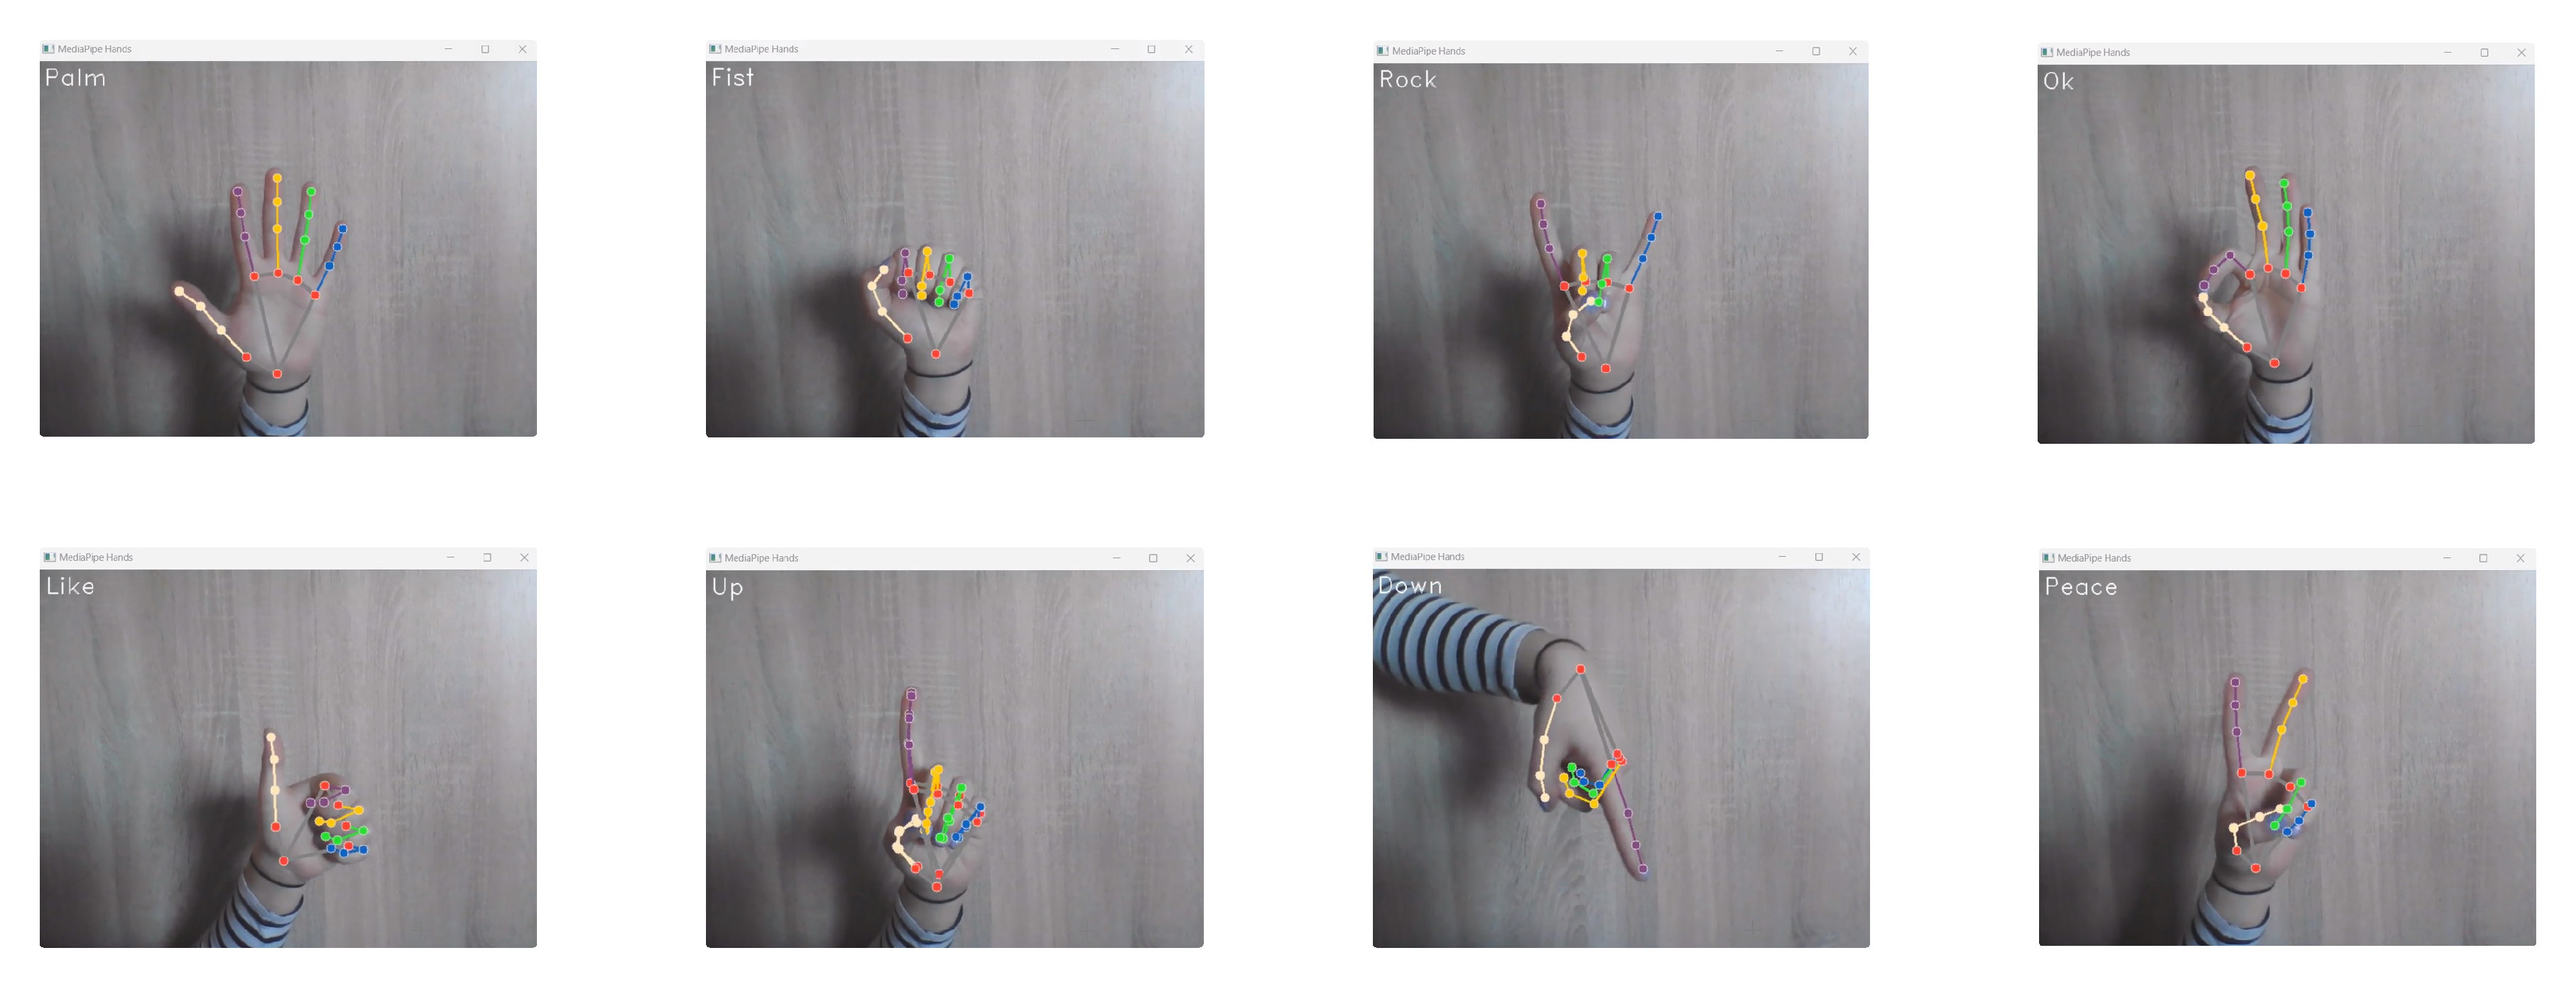
\includegraphics[width = \textwidth]{images/all_gestures.pdf}
	\caption{Gestures used in the project}
	\label{fig:all_gestures}
\end{figure}





\subsubsection{Data Normalization}
The MediaPipe hand landmarks model provides coordinates for hand landmark points based on the position of pixels containing those points in an image. As a result, the coordinates of two images of the same hand sign with different placements in the frame can have significantly different distances between them. This makes it more challenging to train the model.

 To solve this problem, the wrist's landmark point has been considered with coordinates (0,0), and the coordinates of all other landmark points were adjusted accordingly.
First, the coordinates' values of the wrist's landmark point are subtracted from all coordinates' values. 


 Then, the coordinates were normalized to be between 0 and 1 by dividing them by the largest absolute value of the difference. Finally, the normalized coordinates were collected in the landmarks list. The coordinate normalization procedure is shown in Fig \ref{fig:normalization}.
\begin{figure}
	\centering
	\includegraphics[width = 0.85\textwidth]{images/normalise.pdf}
	\caption{Process of normalization of landmark coordinates}
	\label{fig:normalization}
\end{figure}




\section{Gesture Recognition}

The process of recognizing hand gestures as input, mapping them to a representation, and converting them into a purposeful command for devices is known as gesture recognition. The goal is to identify and process explicit hand gestures for output. 
Dynamic gestures refer to a sequence of poses that change over time, while static gestures remain constant. Static hand gestures can be classified based on their temporal relationship and recognized by analyzing features such as spatial position, orientation, contour, and texture. We will focus on recognizing static gestures using a vision-based method.


tu nejake obrazky na classification

\section{Drone Control}






%practice
\chapter{Practical Part}
In our task, we heavily worked with MediaPipe. We used it for data collection, face recognition, and finally gesture recognition. 

\section{Mediapipe}
MediaPipe is a framework used to create machine learning pipelines for time-series data like video and audio. Google initially developed it to process real-time video and audio analysis on YouTube \cite{mediapipe2019blog}. In 2019, the public release allowed researchers and developers to incorporate MediaPipe into their projects. Unlike other machine learning frameworks that require high computing power, MediaPipe can run efficiently on devices with low power, such as Android and IoT devices. It consists of the MediaPipe framework and MediaPipe solutions. The MediaPipe framework is developed using C++, Java, and Objective C programming. MediaPipe solutions include 16 pre-trained TensorFlow and TensorFlow Lite models built on top of the MediaPipe framework for specific use cases.
\subsection*{MediaPipe Hands}
MediaPipe Hands is a solution that tracks hands in real time. The problem of detecting hands is somewhat intricate. The model must be able to recognize hands and it must function across a wide range of hand sizes with a big scale span so it must be robust. It is rather difficult to identify hands based just on their visual traits since hands lack high-contrast patterns.% found on faces, such as those surrounding the lips and eyes.

MediaPipe Hands utilizes a combination of object detection, classification, and regression to recognize and track hands within a given image or video frame. The pipeline consists of two convolutional neural network models: a palm detector and a hand landmark model.


The palm detector is a single-shot detector model that uses an orientated hand-bounding box to locate palms on a whole input image. This is done before landmark detection because it is easier to estimate bounding boxes of rigid objects like palms than detecting hands with articulated fingers. It ignores many aspect ratios and so the bounding boxes are only squared. The model uses both classification (hands, no hands), and object detection (predicting a bounding box around the detected hand), a focal loss \cite{DBLP:journals/corr/abs-1708-02002} It was trained on data, containing 700 images of 14 geographical subregions, from both men and women.


The Hand Landmark Model runs subsequently with the palm detection model and uses regression to precisely localize 21 3D (x, y, z) coordinates within the hand region. Each landmark has a specific location on the hand that can vary within the pixel grid of an image. To capture the exact position, continuous values are used, allowing the model to indicate precisely where each landmark is located on the hand in terms of its x and y (and possibly z) coordinates within the image. The hands move and rotate freely, leading to a wide range of possible positions and orientations for each landmark. Continuous values are used because they make it possible to track hand gestures and movements more precisely. These gestures and movements may involve tiny changes to position and orientation that would be lost in discretized values.
The model is resilient to self-occlusions and partially visible hands, and it learns a consistent internal hand posture representation. The results from the model contain 21 hand landmarks consisting of x, y, and z, a hand flag that indicates the likelihood that a hand is present in the input image, and a binary system of handedness, e.g. left or right hand.
The coordinates x and y for each landmark are normalized \ref{sec:norm} to [0, 1] by image width and height. 

The model was trained both on real-world and synthetic datasets, noting that the wrist point was learned only from synthetic images. More than 30,000 manually annotated real-world images were used and the model is very robust, allowing it to detect and map hand landmark points accurately, even on partially visible hands in most cases. In Figure
\ref{fig:landmark_both_hands} my hands are not facing upfront but the model still finds all the landmarks for both hands. If tracking 2 hands, it also shows which one is left or right with different colors.

For encountering a tracking failure, There was also another model output created for tracking failures. It generates the likelihood that the given crop contains a hand that is reasonably aligned. The detector is triggered to reset tracking if the score falls below a predetermined threshold.

\begin{figure}
	\centering
	\includegraphics[width = 0.5\textwidth]{images/landmarks_both_hands.png}
	\caption{Hand landmarks model output}
	\label{fig:landmark_both_hands}
\end{figure}

\subsubsection*{Data Normalization}\label{sec:norm}
The MediaPipe hand landmarks model provides coordinates for hand landmark points based on the position of pixels containing those points in an image. As a result, the coordinates of two images of the same hand sign with different placements in the frame can have significantly different distances between them. This makes it more challenging to train the model.

To solve this problem, the wrist's landmark point has been considered with coordinates [0,0], and the coordinates of all other landmark points were adjusted accordingly.
First, the coordinates' values of the wrist's landmark point are subtracted from all coordinates' values.

Then, the coordinates were normalized to be between 0 and 1 by dividing them by the largest absolute value of the difference. Finally, the normalized coordinates were collected in the landmarks list. The coordinate normalization procedure is shown in Figure \ref{fig:normalization}.


\begin{figure}
	\centering
	\includegraphics[width = 0.85\textwidth]{images/normalise.pdf}
	\caption{Process of normalization of landmark coordinates}
	\label{fig:normalization}
\end{figure}

\subsection*{MediaPipe Face}
With support for multiple faces and six landmarks (left eye, right eye, nose tip, mouth, left eye region, and right eye region), MediaPipe Face Detection is a quick solution for face detection. Mediapipe BlazeFace is a compact and efficient face detector designed for mobile GPU inference, that serves as its foundation. Because of its real-time performance, the detector can be used with any live viewfinder experience that needs a precise facial region of interest as an input for other task-specific models, like face region segmentation, facial feature or expression classification, and 3D facial int estimation (like MediaPipe Face Mesh). BlazeFace leverages an enhanced tie resolution technique as an alternative to a GPU-friendly anchor mechanism adapted from Single Shot MultiBox Detector (SSD) and a lightweight feature extraction network that is similar to but different from MobileNetV1/V2.


\begin{figure}[ht]
	\centering
	\begin{minipage}{0.5\textwidth}
		\centering
		\includegraphics[width=0.5\textwidth]{images/face_detection_good.png}
		%   \caption{Landmarks for pose estimation model by MediaPipe}
	\end{minipage}% <-- This percentage sign denotes the end of a minipage
	\begin{minipage}{0.5\textwidth}
		\centering
		\includegraphics[width=0.5\textwidth]{images/face_detection.png}
		%   \caption{U-Net segmentation on an image from Oxford-IIIT Pet Dataset (Parkhi et al, 2012).}
	\end{minipage}
	\caption{Outputs of face detection model with different lightings}
	\label{fig:face_detections} % This label can now be used to reference both images together
\end{figure}


\section{Data Collection}
The flow of this project is as follows: the drone flies off, and we process the image that is captured by the drone's camera. Using multiple models for detecting, classifying, and localizing features in the image, after detecting a face, our model returns a prediction of a gesture and the drone executes the corresponding command in real time. The logic of the process is presented in Figure \ref{fig:flowchart}


\begin{figure}
	\centering
	\includegraphics[width = 0.9\textwidth]{images/flowchart.pdf}
	\caption{Logic in the recognition process}
	\label{fig:flowchart}
\end{figure}


In order to make predictions, we had to train our model with data. Since we decided to use hand gestures, we had to collect the data ourselves. After finishing the training, we established drone commands and tested our program.

Although there are many publicly accessible datasets that contain pictures of hand gestures, we chose to collect our own data using the MediaPipe hand-tracking model. To do this, we recorded video footage of various hand gestures being held for a specific duration and moved around to increase diversity. Because the MediaPipe models are open-sourced and many developers use them for various projects, there are also numerous programs available for capturing and labeling gestures, like \cite{opencv_mediapipe_hand_gesture_recognition}. During the recording process, we labeled each gesture by pressing a key. Our dataset includes over 5000 samples, including images of both right and left hands, palms facing forward or backward toward the camera, and various degrees of hand positions captured by the camera.

\begin{figure}
	\centering
	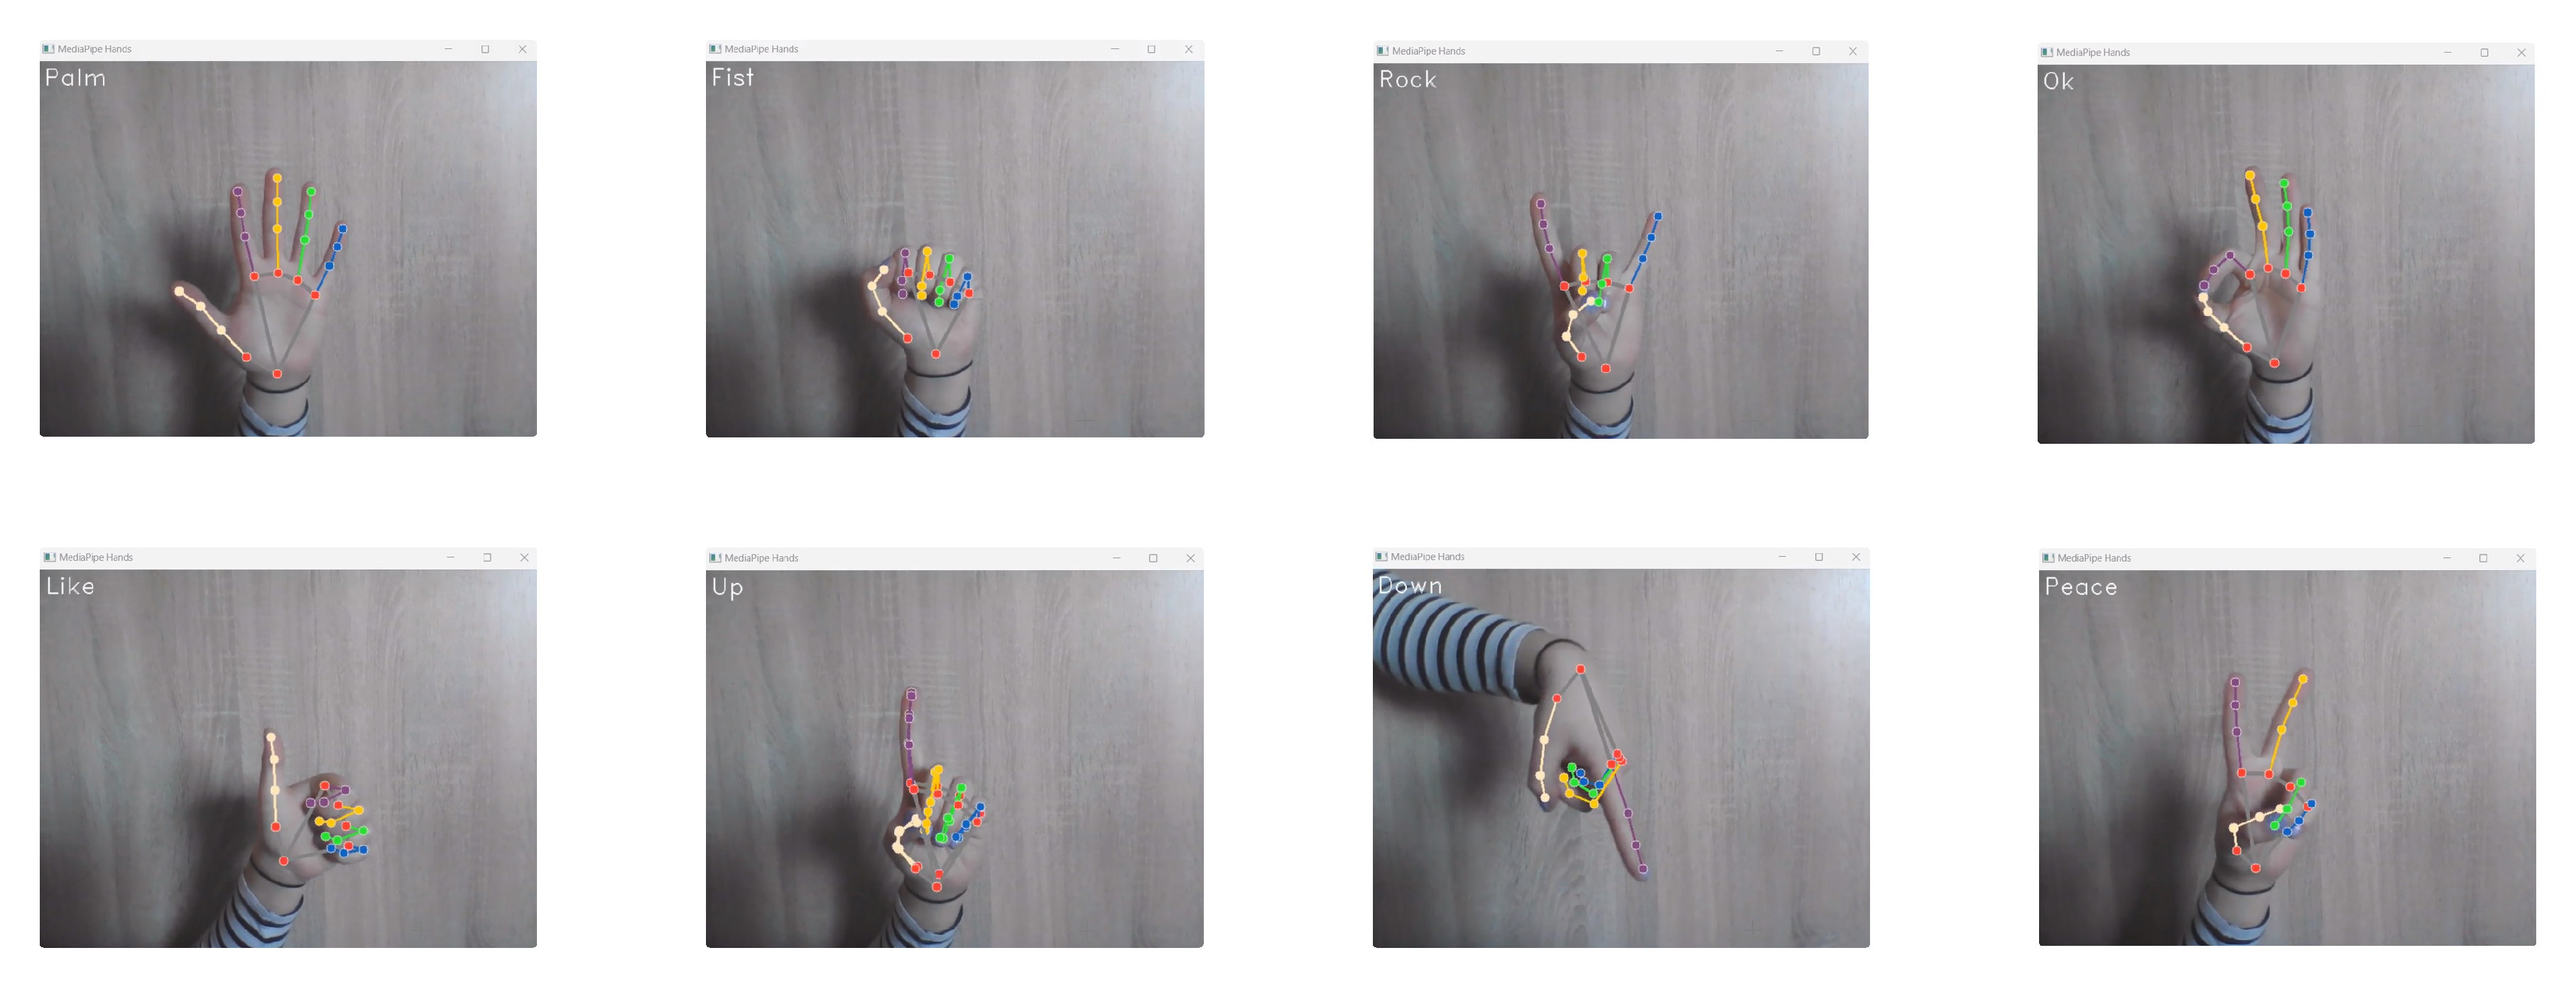
\includegraphics[width = \textwidth]{images/all_gestures.pdf}
	\caption{Gestures used in this project.}
	\label{fig:all_gestures}
\end{figure}


Our final dataset has 8 total classes. It demonstrates the efficacy of the model and minimizes the risk of error commands that could lead to unsafe situations. The gestures are shown in Figure \ref{fig:all_gestures}.


The hand-tracking model used for data collection, outputs x, y, and z coordinates of hand landmark points from images, but only x and y coordinates are necessary for training the final model. Therefore, we eliminated the z coordinates. After normalization \ref{sec:norm}, we stored the remaining x and y coordinates of hand landmarks for various hand signs in a csv file for each hand landmark. The coordinates displayed in Figure \ref{fig:saved_csv} represent the data points used to generate the final dataset and train the final model. The first column denotes the gesture label, the next two columns indicate the coordinates of landmark 0 at the wrist, and so on. Our csv file contains many combinations of landmark coordinates for each gesture.


\begin{figure}[h]
	\centering
	\includegraphics[width = \textwidth]{images/gesture_laandmarks-cropped.pdf}
	\caption{A selection of the saved csv file}
	\label{fig:saved_csv}
\end{figure}


\section{Model}
\begin{figure}[ht]
	\centering
	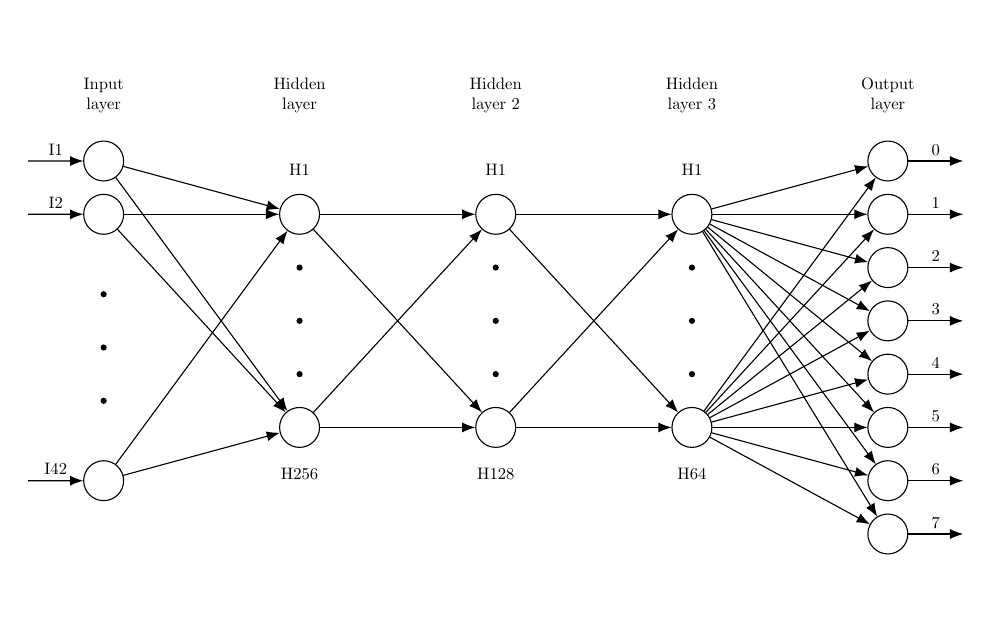
\begin{tikzpicture}[
		scale = 0.7,
		every node/.style={scale=0.6},
		plain/.style={
			draw=none,
			fill=none,
		},
		cir/.style={
			draw,
			circle,
			inner sep=8.5pt
		},
		dot/.style={
			draw,
			shape=circle,
			minimum size=3pt,
			inner sep=0,
			fill=black
		},
		net/.style={
			matrix of nodes,
			nodes={
				draw,
				circle,
				inner sep=8.5pt
			},
			nodes in empty cells,
			column sep=1cm,
			row sep=-5pt
		},
		arrow/.style={-Latex}
		]
		\matrix[net] (mat)%10x5
		{
			|[plain]| \parbox{1.5cm}{\centering Input\\layer}
			& |[plain]| \parbox{1.5cm}{\centering Hidden\\layer}
			& |[plain]| \parbox{1.5cm}{\centering Hidden\\layer 2}
			& |[plain]| \parbox{1.5cm}{\centering Hidden\\layer 3}
			& |[plain]| \parbox{1.5cm}{\centering Output\\layer} \\
			|[cir]| &           |[plain]| &     |[plain]| &         |[plain]| &             |[cir]| \\
			|[plain]| &         |[plain]| &     |[plain]| &         |[plain]| &               |[plain]| \\
			|[cir]| &           |[cir]| &       |[cir]| &         |[cir]| &             |[cir]| \\
			|[plain]| &         |[plain]| &       |[plain]| &           |[plain]| &               |[plain]| \\
			|[plain]| &         |[dot]| &       |[dot]| &           |[dot]| &               |[cir]| \\
			|[dot]| &           |[plain]|   &     |[plain]| &           |[plain]| &               |[plain]| \\
			|[plain]| &         |[dot]| &     |[dot]| &         |[dot]| &             |[cir]| \\
			|[dot]| &           |[plain]| &       |[plain]| &           |[plain]| &               |[plain]| \\
			|[plain]| &         |[dot]| &     |[dot]| &         |[dot]| &             |[cir]| \\
			|[dot]| &           |[plain]| &     |[plain]| &         |[plain]| &             |[plain]| \\
			|[plain]| &         |[cir]| &       |[cir]| &           |[cir]| &               |[cir]| \\
			|[plain]| &         |[plain]| &     |[plain]| &         |[plain]| &             |[plain]| \\
			|[cir]| &           |[plain]| &     |[plain]| &         |[plain]| &             |[cir]| \\
			|[plain]| &         |[plain]| &     |[plain]| &         |[plain]| &             |[plain]| \\
			|[plain]| &         |[plain]| &     |[plain]| &         |[plain]| &             |[cir]| \\
			|[plain]| &         |[plain]| &     |[plain]| &         |[plain]| &             |[plain]| \\
		};
		
		% Connect the 'cir' nodes from Input Layer to Hidden Layer 1
		\draw[arrow] (mat-2-1) -- (mat-4-2);
		\draw[arrow] (mat-2-1) -- (mat-12-2);
		\draw[arrow] (mat-4-1) -- (mat-12-2);
		\draw[arrow] (mat-4-1) -- (mat-4-2);
		\draw[arrow] (mat-14-1) -- (mat-4-2);
		\draw[arrow] (mat-14-1) -- (mat-12-2);
		
		% Connect the 'cir' nodes from Hidden Layer 1 to Hidden Layer 2
		\draw[arrow] (mat-4-2) -- (mat-4-3);
		\draw[arrow] (mat-4-2) -- (mat-12-3);
		\draw[arrow] (mat-12-2) -- (mat-12-3);
		\draw[arrow] (mat-12-2) -- (mat-4-3);
		
		
		% Connect the 'cir' nodes from Hidden Layer 2 to Hidden Layer 3
		\draw[arrow] (mat-4-3) -- (mat-4-4);
		\draw[arrow] (mat-4-3) -- (mat-12-4);
		\draw[arrow] (mat-12-3) -- (mat-12-4);
		\draw[arrow] (mat-12-3) -- (mat-4-4);
		
		% Connect the 'cir' nodes from Hidden Layer 3 to Output Layer
		\draw[arrow] (mat-4-4) -- (mat-2-5);
		\draw[arrow] (mat-4-4) -- (mat-4-5);
		\draw[arrow] (mat-4-4) -- (mat-6-5);
		\draw[arrow] (mat-4-4) -- (mat-8-5);
		\draw[arrow] (mat-4-4) -- (mat-10-5);
		\draw[arrow] (mat-4-4) -- (mat-12-5);
		\draw[arrow] (mat-4-4) -- (mat-14-5);
		\draw[arrow] (mat-4-4) -- (mat-16-5);
		
		\draw[arrow] (mat-12-4) -- (mat-2-5);
		\draw[arrow] (mat-12-4) -- (mat-4-5);
		\draw[arrow] (mat-12-4) -- (mat-6-5);
		\draw[arrow] (mat-12-4) -- (mat-8-5);
		\draw[arrow] (mat-12-4) -- (mat-10-5);
		\draw[arrow] (mat-12-4) -- (mat-12-5);
		\draw[arrow] (mat-12-4) -- (mat-14-5);
		\draw[arrow] (mat-12-4) -- (mat-16-5);
		
		
		% Labels for cir nodes
		% Incoming arrows with labels for the input layer 'cir' nodes
		\draw[arrow] ([xshift=-1cm]mat-2-1.west) -- (mat-2-1) node[above, midway] {I1 };
		\draw[arrow] ([xshift=-1cm]mat-4-1.west) -- (mat-4-1) node[above, midway] {I2 };
		\draw[arrow] ([xshift=-1cm]mat-14-1.west) -- (mat-14-1) node[above, midway] {I42 };
		
		\node[above=0.5cm of mat-5-2] (hidden11) {H1};
		\node[above=0.7cm of mat-17-2] (hidden12) {H256};
		
		\node[above= 0.5cm of mat-5-3] (hidden21) {H1};
		\node[above= 0.7cm of mat-17-3] (hidden22) {H128};
		
		\node[above=0.5cm of mat-5-4] (hidden31) {H1};
		\node[above=0.7cm of mat-17-4] (hidden32) {H64};
		
		\draw[arrow] (mat-2-5.east) -- ([xshift=1cm]mat-2-5.east) node[above, midway] {0};
		\draw[arrow] (mat-4-5.east) -- ([xshift=1cm]mat-4-5.east) node[above, midway] {1};
		\draw[arrow] (mat-6-5.east) -- ([xshift=1cm]mat-6-5.east) node[above, midway] {2};
		\draw[arrow] (mat-8-5.east) -- ([xshift=1cm]mat-8-5.east) node[above, midway] {3};
		\draw[arrow] (mat-10-5.east) -- ([xshift=1cm]mat-10-5.east) node[above, midway] {4};
		\draw[arrow] (mat-12-5.east) -- ([xshift=1cm]mat-12-5.east) node[above, midway] {5};
		\draw[arrow] (mat-14-5.east) -- ([xshift=1cm]mat-14-5.east) node[above, midway] {6};
		\draw[arrow] (mat-16-5.east) -- ([xshift=1cm]mat-16-5.east) node[above, midway] {7};
		
		% ... (rest of your output labels)
		
		
	\end{tikzpicture}
	\caption{Neural network architecture.}
	\label{fig:neural_network}
\end{figure}

The model we used for gesture recognition is a fully connected feedforward neural network. The model is adjusted to work with data output by KeyPointClassifier. KeyPointClassifier is a class that processes data of MediaPipe Hands models. The data are then sent to our gesture classifier.


%\begin{figure}
%	\centering
%	\includegraphics[width = 0.65\textwidth]{images/model_summ.png}
%	\caption{Configuration of the used feedforward neural network}
%	\label{fig:layers}
%\end{figure}
The following is a report on training our neural network with the data. We utilized a model, which comprises one input layer and one output layer, along with five hidden layers consisting of three dense layers and two dropout layers. The sequential application of dropout and dense layers with ReLU activation acts as a mechanism to prevent overfitting while allowing the model to make nonlinear mappings. The output layer of the neural network comprises neurons equivalent to the number of hand gestures it can recognize - 8. The configuration of the model is depicted in Figure \ref{fig:layers}. The was trained with a dataset split into training and testing sets, and was designed using the Adam optimizer, which is efficient and appropriate for training models with large data and parameters. The Sparse Categorical Crossentropy loss function was utilized to evaluate the loss between predicted and actual labels, while accuracy was used as the evaluation metric to determine how frequently the prediction matches the actual label. The training was halt by early stopping when the validation loss stopped to decrease and then converted into TensorFlow Lite to reduce its size. Initially, the training model was set to have only four hidden layers (2 dense layers). However, the training accuracy failed to exceed 90\%. Consequently, we updated the model to have five hidden layers (with 3 dense layers), without any other modifications and obtained satisfactory results. The training accuracy achieved was 99.48\%, and the calculated loss was 0.031.





\section{Results}

To perform a quantitative analysis of the test dataset, we employed the  \text{classification\_report} and  \text{confusion\_matrix} libraries from scikit-learn. The \text{classification\_report} library produced an assessment report of our model with accuracy, precision, recall, and F1 score matrices. Additionally, the support matrix represents the model's real-time recognition performance.


\begin{figure}
	\centering
	\includegraphics[width = 0.65\textwidth]{images/classific_report.png}
	\caption{Classification report of the model}
	\label{fig:report}
\end{figure}


Precision is the ratio of correctly predicted positive observations to the total predicted positive observations. 

The accuracy matrix calculates the number of correctly predicted labels by the model from the entire dataset (Eq.\ref{eq:accuracy}). 
The precision matrix measures the model's accuracy out of the predicted positives. It calculates the number of actual positives in the predicted positives and is an excellent measure to consider when the False Positive (FP) cost is high. Equation \ref{eq:precision} depicts the mathematical formula of the precision matrix.

The recall matrix measures the number of predictions our model correctly labels as positives. It is a measure considered when false negatives have high costs. The mathematical formulation of the recall matrix is Equation \ref{eq:recall}. 

The F1 score is calculated by combining both precision and recall, as shown in Equation \ref{eq:f1_score}. It is their harmonic mean.

Support is the number of samples in each class. 
The macro-average of precision, recall and F1-score demonstrates the system's average performance across all classes, while the weighted average takes into account the class imbalance by weighting the metrics based on the number of samples in each class. Additionally, the loss value of 0.0310 (not shown) indicates how efficiently the model is minimizing its errors during training.

The classification report of the implemented model in detail is shown in Figure \ref{fig:report}. 


\begin{equation}
	\text{accuracy} = \frac{TP + TN}{TP + TN + FP +FN}
	\label{eq:accuracy}
\end{equation}

\begin{equation}
	\text{precision} = \frac{TP}{TP + FP}
	\label{eq:precision}
\end{equation}
\begin{equation}
	\text{recall} = \frac{TP}{TP + FN}
	\label{eq:recall}
\end{equation}

\begin{equation}
	\text{F1 score} = \frac{2 P  R}{P+ R} 
	\label{eq:f1_score}
\end{equation}

In the equations (\ref{eq:accuracy}), (\ref{eq:precision}), (\ref{eq:recall}), and (\ref{eq:f1_score}), TP, TN, FP, and FN represent True Positive, True Negative, False Positive,
and False Negative, respectively.

The confusion matrix is a key performance metric used in machine learning, particularly in classification tasks. By utilizing the scikit-learn library in Python, one can create a confusion matrix. To conduct our experiment on predicting hand gestures, we obtained and pre-processed the necessary datasets. The confusion matrix was then utilized to evaluate the accuracy of our model, which is illustrated in Figure \ref{fig:confusion_matrix}. The x-axis represents predicted labels, while the y-axis represents actual labels.

Through the confusion matrix, we can pinpoint which gestures are being incorrectly recognized. For instance, we observed that gesture 2 was misinterpreted as gesture 6 a total of 11 times. We can further calculate the recall of gesture 2 utilizing Equation \ref{eq:recall2}:

\begin{equation}
	\text{recall(2)} = \frac{545}{545 + 11}
	\label{eq:recall2}
\end{equation}



\begin{figure}
	\centering
	\includegraphics[width = 0.65\textwidth]{images/confusion_matrix.pdf}
	\caption{Confusion matrix of the model}
	\label{fig:confusion_matrix}
\end{figure}

The system's performance is satisfactory, with almost perfect precision, recall, and F1-score in most classes, as well as high accuracy and weighted average.

\subsection*{Demos}
In the beginning, we tried to recognize only 4 gestures.

\subsection{Drone Implementation}

The Tello drone is a compact quadcopter equipped with a vision positioning system and an onboard camera. It can be operated through a laptop computer via Wi-Fi or a smartphone using 2.4 GHz. The Tello library, which can be easily accessed with Python, contains a range of built-in functions for managing communication with the drone, handling state changes, and controlling the drone through a series of events.

Our program prompts the Tello drone to begin executing commands after a key press and identifies a gesture every 5 seconds. This allows for the comfortable execution of a command before recognizing the next one. After tweaking speeds and sleep times, the Tello drone executed the received commands rapidly and consistently.

Table \ref{tab:gesture_commands} lists the commands used in our project, which were assigned to the labels of our gestures. The gestures we utilized can be found in Figure \ref{fig:all_gestures}.

\begin{table}[ht]
	\centering
	\begin{tabular}{ll}
		\toprule
		Gesture Label & Command \\
		\midrule
		0 - Palm& Move along the y-axis (forward velocity) \\
		1 - Fist& Move along -y-axis (backward velocity) \\
		2 - Rock& Flip forward (upward velocity) \\
		3 - OK & Take-off or land (depending on whether in flight or landed) \\
		4 - Peace& Takes a picture (saves in png) \\
		5 - Like& Rotate 360$^\circ$ \\
		6 - Up& Move up (ascending velocity) \\
		7 - Down & Move down (descending velocity)\\
		\bottomrule
	\end{tabular}
	\caption{Gesture commands for drone control}
	\label{tab:gesture_commands}
\end{table}



In addition, if we are not recognizing any gesture, the drone is ready to land on the palm. Because the drone can execute most of the commands only while flying, it takes off at the start of the program. It can also take off with gesture 4, so the program doesn't have to be reset.









% conclusions
\chapter{Conclusions}
In this project, we have achieved touchless interaction between the drone and our hands. We implemented a machine learning model, specifically MediaPipe, for hand tracking. Our gesture recognition model underwent training and testing, and the confusion matrix presents its accuracy. The process is composed of 5 steps: 
\begin{enumerate}[label=\Roman*.]
    \item Drone capturing an image
    \item Image processing via OpenCV
    \item Gesture recognition
    \item Gesture - command conversion
    \item Command execution
  
\end{enumerate}
 Gesture recognition is used in various sectors, including smart home automation and the medical field. It mainly focuses on human-machine interaction. The system receives input images from a drone camera connected to the device. The main goal of this project is to propose a real-time system with high accuracy. 
In summary, the project demonstrates how we can control a drone in an entertaining and educational way. 
\begin{figure}
	\centering
	\includegraphics[width = \textwidth]{images/steps.pdf}
	\caption{Steps of the process}
	\label{fig:conclusion}
\end{figure}
\clearpage

% Appendices (Prílohy) comment by "%" if not neccesary
\appendix
 \chapter{Resumé}
 \label{ch:resume}
Táto bakalárska práca sa zaoberá teoretickými a praktickými aspektmi strojového učenia a jeho aplikáciami v počítačovom videní, neurónových sieťach a rozpoznávaní gest. V teoretickej časti sa zameriava na preskúmanie rôznych techník učenia, ako je učenie s učiteľom, či bez učiteľa, no najmä metódami počítačového videnia, ako sú klasifikácia, detekcia a segmentácia.\newline
 Počítačové videnie využíva klasifikáciu na rozpoznanie vlastností objektov, z ktorých potom určuje do ktorých kategórií tieto objekty patria. Pre samotnú klasifikáciu platí všeobecný postup: predspracovanie obrazu -> extrakcia čŕt -> klasifikácia objektov. Klasifikáciu možno taktiež rozdeliť na binárnu, kde výstupom je jedna z dvoch možností, multi-class, kde výstup je výber z viac ako dvoch možností, klasifikáciu viacerých značiek (multilabel), kde výstupu možno priradiť viac ako jednu možnosť alebo hierarchickú klasifikáciu, kedy sa triedy radia do hierarchickej štruktúry na základe podobnosti. Triedy nižších úrovní sú konkrétnejšie a detailnejšie ako triedy vyšších úrovní. Pri detekcii objektov, platí že jej výstupom sú ohraničujúce obdĺžniky, ako aj trieda do ktorej objekt patrí. Detekcii veľmi podobnou úlohou je segmentácia, kde princípom je nájdenie a oddelenie jednotlivých objektov od pozadia s presnosťou na pixely.\newline
Ďalej sa v teoretickej časti venujeme neurónovým sieťam. Neurónová sieť je sieť pospájanýh neurónov, medzi ktorými sa posúvajú informácie.	Pri doprednej sieti sa informácia posúva vpred, od vstupných neurónov k výstupným, a to cez skryté vrstvy neurónov. Vstupnú vrstvu tvoria priamo dáta vlastností, zatiaľ čo údaje získané z výstupnej vrstvy slúžia ako základ pre klasifikáciu vstupných dát. Neurón má niekoľko vstupov  ($x_1, x_2, ..., x_n$) a jeden výstup $\hat{y}$, pričom každý vstup má svoju „váhu“, teda dopredu dané číslo, ktoré vyjadruje významnosť jednotlivých vstupov. Neurón vezme vážený súčet vstupov a aplikuje naňho aktivačnú funkciu. Aktivačné funkcie sú základným prvkom neurónových sietí a poskytujú im nelinearitu potrebnú pre modelovanie zložitých vzorcov. Aktivačná funkcia môže byť rôzna, ako napríklad sigmoid, softmax alebo ReLU (Rectified Linear Unit). Voľba aktivačnej funkcie výrazne ovplyvňuje rýchlosť, s akou algoritmus učenia dosahuje konvergenciu. Jej správny výber je podmienený štruktúrou a charakteristikami dát a účelom modelu. Aktivačné funkcie predstavujú matematické vzorce, ktoré určujú výstupy modelu. \newline
																																			


% Resumé v slovenčine, sa píše v prípade, že záverečná práca ja napísaná v 
% anglickom jazyku. Rozsah resumé tvorí 5-10\% rozsahu diplomovej práce.

%----------------------------------------------------------------%
%  The Backmatter !! Do NOT change the structure!!               %
%----------------------------------------------------------------%

%\nocite{*}
% Bibliography to TOC
% do not remove
\backmatter

\providebibliography
\bibliography{bibfile}

%----------------------------------------------------------------%
%   The end of the document                                      %
%----------------------------------------------------------------%
\end{document}

